\begin{scanpage}{0160}{142}
\begin{center}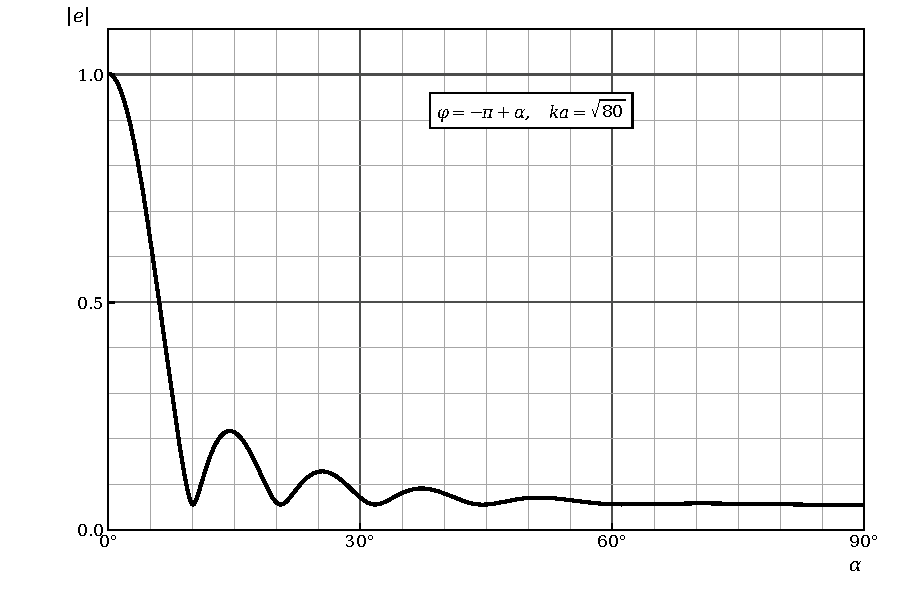
\includegraphics[width=.55\linewidth]{images/recreated/c-0160-fig62.pdf}\par
Figure 62. The same as Figure 59 when $\phi=-\pi+\alpha$.
\end{center}
In accordance with \S~12, the fringing field in the plane $\phi=\pm\pi/2$ is described (when $R\gg ka^2$) by the equations
\[
\left.\begin{aligned}E_\varphi=-H_\vartheta={}&\frac{iaE_{0\varphi}}2\bigl\{[f(2,\delta)-f(1,\delta)]J_1(\zeta)\\&+i[f(2,\delta)+f(1,\delta)]J_2(\zeta)\bigr\}\frac{e^{ikR}}R,\\
H_\varphi=E_\vartheta={}&\frac{iaH_{0\varphi}}2\bigl\{[g(2,\delta)-g(1,\delta)]J_1(\zeta)\\&+i[g(2,\delta)+g(1,\delta)]J_2(\zeta)\bigr\}\frac{e^{ikR}}R.
\end{aligned}\right\}\tag{24.02}
\]
These expressions are valid when $\vartheta<\pi/2$ and $\gamma<\pi/2$. The quantities included in them are determined by the relationships:
\[
\left.\begin{aligned}f(1,\delta)&=\frac{\cos\frac{\delta+\vartheta}{2}-\sin\frac{\delta-\vartheta}{2}}{\sin\delta-\sin\vartheta},\\
f(2,\delta)&=-\frac{\cos\frac{\delta+\vartheta}{2}+\sin\frac{\delta-\vartheta}{2}}{\sin\delta-\sin\vartheta},\\
g(1,\delta)&=-f(2,\delta),\qquad g(2,\delta)=-f(1,\delta),
\end{aligned}\right\}\tag{24.03}
\]
\[
\zeta=ka(\sin\vartheta-\sin\delta).\tag{24.04}
\]
\end{scanpage}
